\section{效率修正}
\label{chap:efficiency}
如\ref{chap:raw_signal}所讨论的那样,对于原初信号我们需要对其进行STAR探测器的效率修正才能得到STAR接收度下的双电子谱。这里所说的效率指的是电子对在STAR接收度下的探测效率,因为对一个电子对来说,正负电子的测量是两个独立的事件,所以电子对的效率就等于正负电子的探测效率直接相乘。对单个电子来说,其探测效率又等于所有探测器探测效率和电子鉴别的判选条件的效率的乘积。双电子谱修正方法和效率的计算公式如式\ref{eq:eff}所示。
\begin{equation}
    \begin{split}
        N_{STAR~acc.} = \frac{ N_{raw~signal} }{ \epsilon_{pair~eff.} }\\
        \epsilon_{pair~eff.} = \epsilon_{e^{+}}\times\epsilon_{e^{-}}\\
        \epsilon_{e} = \epsilon_{TPC}\times\epsilon_{TOF}\times\epsilon_{eID}
    \end{split}
\label{eq:eff}
\end{equation}
其中$\epsilon_{pair~eff.}$为电子对探测效率,为 \eplus 与 \eminus 的效率乘积。$\epsilon_{TPC}$, $\epsilon_{TOF}$和$\epsilon_{eID}$分别为时间投影室径迹重建效率、飞行时间探测器探测效率以及电子鉴别效率。这几项将会在接下来的几个小节当中分别讨论。

\subsection{时间投影室径迹重建效率}
在\ref{chap:track_selection}中已经提到过在本分析当中用到的保证径迹重建质量的判选条件。其中和时间投影室相关的包括nHitsFit、nHitsDedx、nHitsFit/nHitsDedx和DCA这几个判选条件。时间投影室径迹重建效率具体的计算公式如式\ref{eq:TPC_eff}所示。又因为时间投影室作为STAR的主探测器,并没有其他的探测器可以提供给我们粒子到达时间投影室之前 的信息,只能通过模拟的手段来得到时间投影室的径迹重建效率。

在STAR实验中,这种模拟的方式被称作embedding。其方法是将蒙特卡洛(Monte Carlo,MC)模拟得到的径迹信息和实际数据混合在一起后再进行时间投影室的径迹重建。就可以得到模拟径迹经过时间投影室重建之前和之后的数量比,从而计算时间投影室径迹重建的效率。在这个过程中,模拟径迹会被随机分配到所有的run当中,每个run中混入的模拟径迹数占总径迹数的百分比固定,以期能更好地反应整个取数过程中时间投影室的平均效率。对于时间投影室本身,端盖部分的支撑结构会带来在$\phi$方向上的死区,这就导致效率在不同的$\phi$方向并不是均匀分布的。在不同的$\eta$和 \pt 区间中也会因为接收度的不同带来一定的效率差别。所以对于不同的\pt 、 $\eta$、 $\phi$,区间,并不能简单的对效率进行平均,这样会抹除掉因为探测器死区和接收度带来的效率差别。所以在计算时间投影室效率的时候,所有的数据根据$\eta$, $\phi$的不同被分为 10($\eta$) $\times$ 36($\phi$)个区间,在每个区间内得到探测效率随着\pt 变化的效率。时间投影室的径迹重建效率除了在不同的接收度区间有差别,也会因为粒子留下的击中密度变化带来探测效率的变化,这样在不同的中心度下探测效率也会发生改变,对于不同的中心度,探测效率需要分别计算。图\ref{fig:TPCTracking} 展示了在不同中心度下时间投影室的径迹重建效率随着\pt 变化的表现,图中对不同的$\eta$, $\phi$区间进行了积分,在具体计算时仍会用到像上文中提到的那样在不同的$\eta$, $\phi$分别计算效率。
\begin{equation}
    \label{eq:TPC_eff}
    \epsilon_{TPC} = \frac{ nTracks( N_{HitsFit} \geq 20~\&\&~\frac{N_{HitsFit}}{N_{HitsPoss}}~\&\&~N_{HitsPoss}\geq15~\&\&~dca\leq1~\&\&~|\eta| < 1 ) }{nTracks(|\eta| < 1)}
\end{equation}

\begin{figure}[htb]
    \begin{center}
    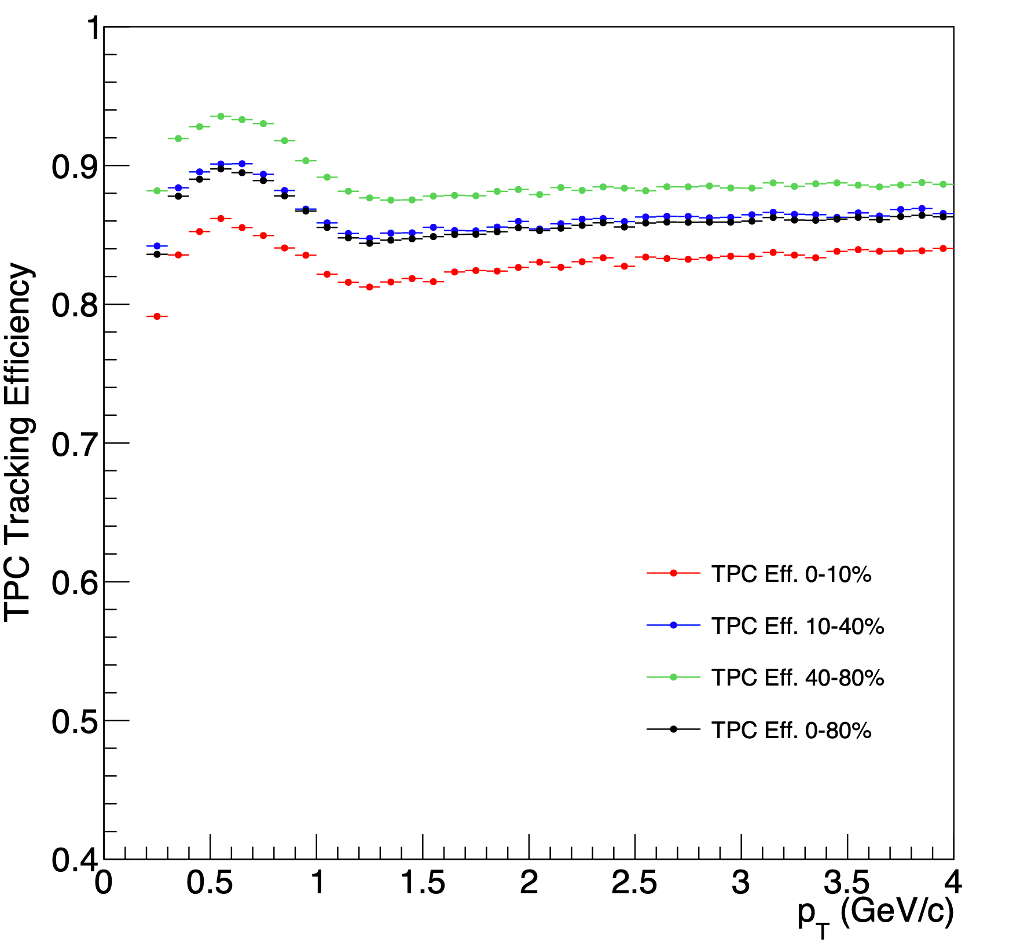
\includegraphics[width=0.75\textwidth,clip]{figures/Chapter4/TPCTracking.png}
    \end{center}
    \caption[不同中心度下时间投影室径迹重建效率示意图]{不同中心度下时间投影室径迹重建效率示意图,不同颜色的点为不同中心度下的径迹重建效率,图中所示效率为对所有$\eta$, $\phi$区间积分后的效率}
    \label{fig:TPCTracking}
\end{figure}

\subsection{飞行时间探测器探测效率}
在\ref{chap:TOF}中已经提到,飞行时间探测器被安装在时间投影室的外部,粒子穿过整个时间投影室后才会打到飞行时间探测器上。这样就可以用时间投影室作为参考探测器,利用真实数据来计算飞行时间探测器的探测效率。即计算时间投影室探测到的粒子和这些粒子被飞行时间探测器探测到的数目之间的比值。具体计算公式如下:
\begin{equation}
    \epsilon_{TOF} = \frac{ nTracks(TOF~Matched, \beta > 0) }{ nTracks(TPC) }
\end{equation}

其中nTracks (TOF Matched)为时间投影室探测到的并且击中飞行时间探测器并被其探测到的径迹, nTracks(TPC)为时间投影室探测到的径迹数。为了更好的反应接收度对效率的影响,和TPC探测效率类似,所有数据根据 $\eta$, $\phi$的不同, 10($\eta$) $\times$ 36($\phi$)个区间,在每个区间得到随 \pt 变化的效率。但因为电子在重离子对撞中每个事例的产生数目较少,纯电子样本没有足够的统计量来进行分$\eta$、 $\phi$区间的效率计算。所以在本分析当中,电子的飞行时间探测器效率是通过计算\piplus 和 \piminus 在各个不同的$\eta$、$\phi$区间内的效率再添加一个修正因子来修正电子和$\pi$之间的效率差别的方式得到的。这个修正因子为电子/正电子和$\rm{\pi^- / \pi^+}$效率之间的比值,同样因为统计的原因这个比值在不同的$\eta$、$\phi$区间内均为一个相同的随着 \pt 变化的因子。图\ref{fig:TOF_match_eff}为0-80\%中心度下正负电子和$\rm{\pi^- / \pi^+}$的飞行时间探测器探测效率随$p_T$变化的比值示意图,图\ref{fig:pi_e_ratio}为前文中提到的修正因子的示意图。

\begin{figure}[htb]
    \centering
    \begin{subfigure}[b]{0.47\textwidth}
        \centering
        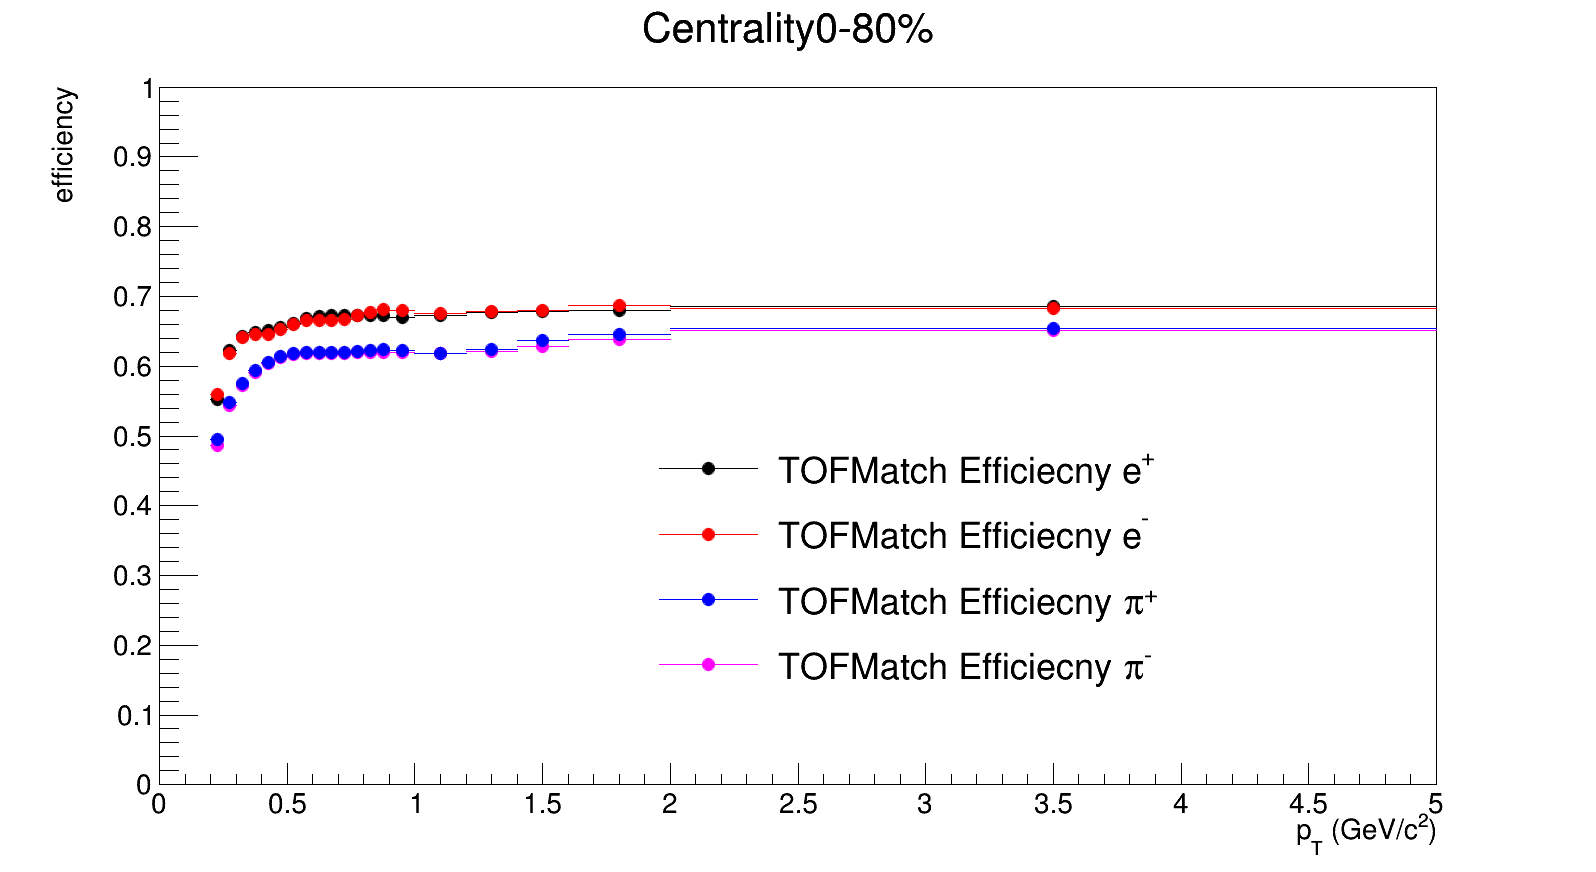
\includegraphics[width=\textwidth,clip]{figures/Chapter4/Eff_Centrality080.png}
        \caption{}
        \label{fig:TOF_match_eff}
    \end{subfigure}
    \hfill
    \begin{subfigure}[b]{0.47\textwidth}
        \centering
        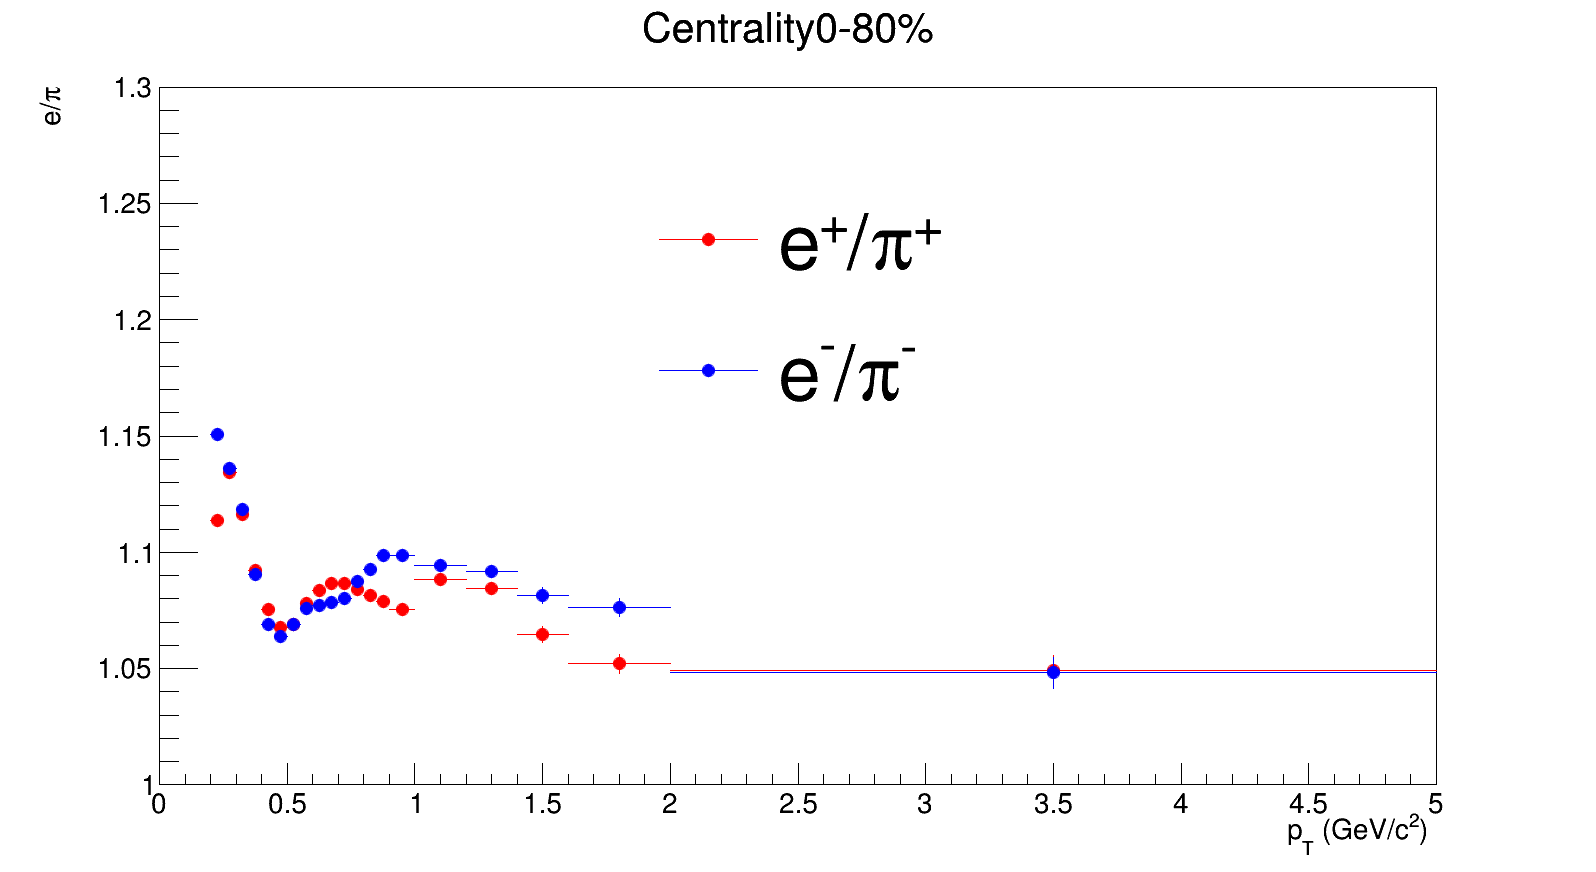
\includegraphics[width=\textwidth,clip]{figures/Chapter4/Ratio_Centrality080.png}
        \caption{}
        \label{fig:pi_e_ratio}
    \end{subfigure}
       \caption[飞行时间探测器匹配效率]{图\ref{fig:TOF_match_eff}为0-80\%中心度下正负电子和正负$\pi$介子的飞行时间探测器匹配效率。图\ref{fig:pi_e_ratio}为正负电子和正负$\pi$介子的效率差别}
       \label{fig:TOFEff}
\end{figure}

\subsection{电子鉴别效率}

本分析当中是通过结合时间投影室测量得到的能量损失信息和飞行时间探测器测量到的粒子飞行速度来进行粒子鉴别的,其判选条件已经在\ref{ch:eID}一节中进行过讨论。这两个判选条件的效率通过分析纯电子数据样本得到。纯光子样本的获取方式和\ref{chap:pruity}中得到纯电子数据样本的方式类似,区别在于计算对应判选条件的效率时纯电子样本选取时不再添加对应的电子鉴别判选条件。对于 \nSigmaE 的判选条件,0-80\%中心度下的结果如图\ref{fig:nSigmaE_cut_eff}所示,通过拟合的方法来最后确定不同动量下的效率。其中拟合的一倍$\sigma$置信区间被用来作为系统误差。对于$1/\beta$的判选条件,在得到纯电子样本之后会通过通过拟合整个分布和bin counting两种方式分别计算$1/\beta$的效率,这两种方式计算得到的效率之间的差别被用作系统误差。

\begin{figure}[htb]
    \centering
    \begin{subfigure}[b]{0.47\textwidth}
        \centering
        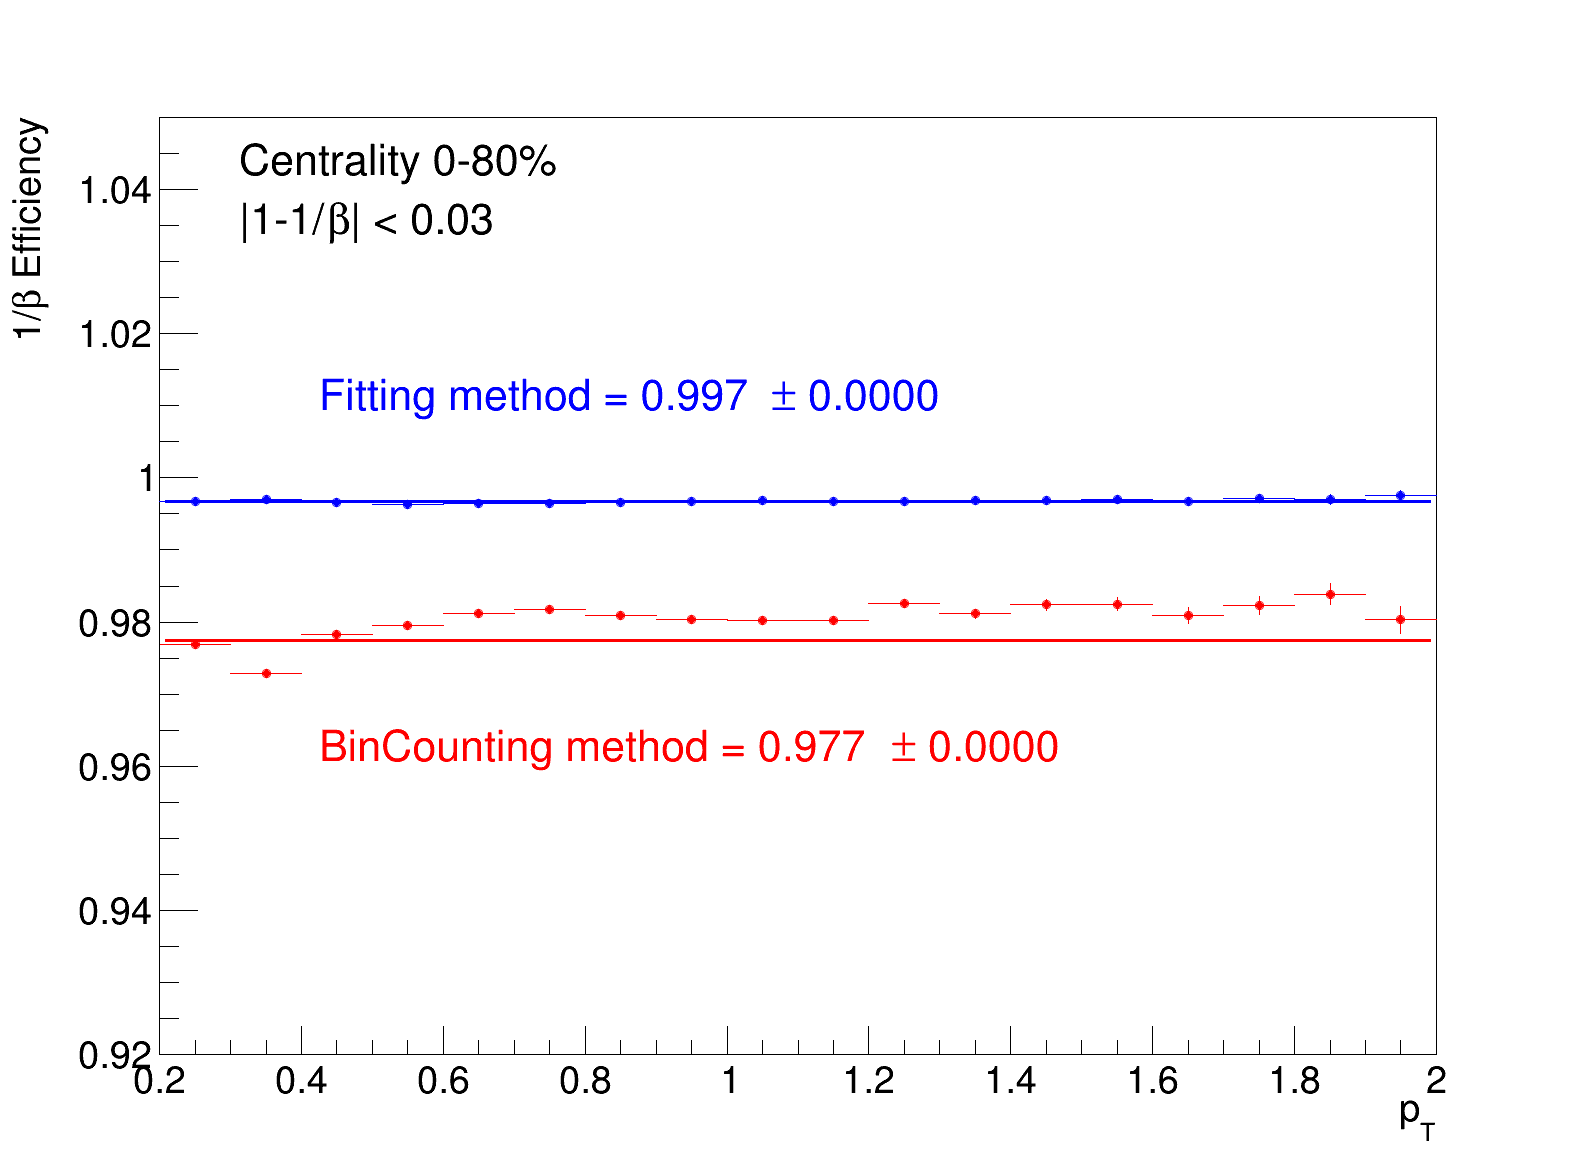
\includegraphics[width=\textwidth,clip]{figures/Chapter4/beta_cut_eff_080.png}
        \caption{}
        \label{fig:beta_cut_eff_080}
    \end{subfigure}
    \hfill
    \begin{subfigure}[b]{0.47\textwidth}
        \centering
        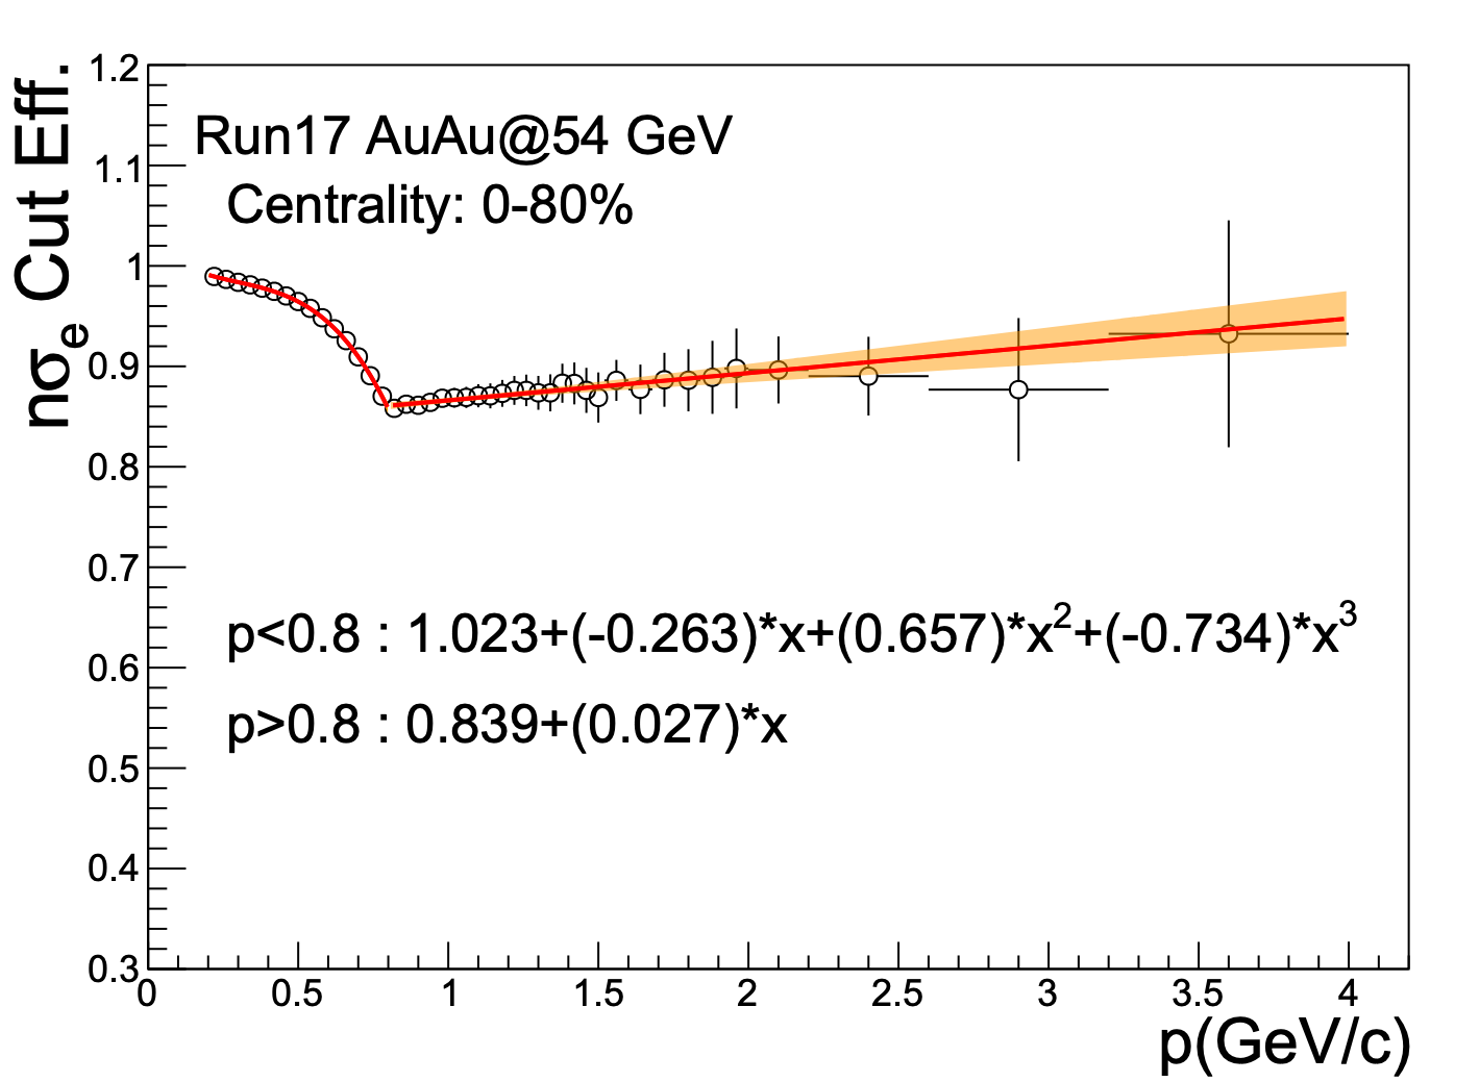
\includegraphics[width=\textwidth,clip]{figures/Chapter4/nSigmaE_cut_eff.png}
        \caption{}
        \label{fig:nSigmaE_cut_eff}
    \end{subfigure}
       \caption[电子鉴别判选条件效率示意图]{图\ref{fig:beta_cut_eff_080}为0-80\%中心度下1/$\beta$的电子鉴别效率,其中两种不同的方法计算的效率的误差。图\ref{fig:nSigmaE_cut_eff}为0-80\%中心度下多高斯拟合得到的$n\sigma_{e}$判选条件效率并进行拟合。其中在$\rm{p > 0.8 GeV}$前后分别用不同曲线拟合,拟合方程在图中列出。}
       \label{fig:TOFEff}
\end{figure}

\subsection{双电子效率修正}
\label{chap:pair_eff}

因为最后我们是得到的双电子谱,所以在最后进行效率修正的时候我们需要的是双电子对的重建效率。在本分析当中,电子对在二维空间($p_T~-~M_{ee}$平面)上重建效率是通过蒙特卡洛模拟(Monte Carlo Simulation)的方法计算得到的。而对于双电子的来源,我们有两种不同的模拟方法:
\begin{itemize}
    \item[1.]虚光子模拟:在这种方法中由虚光子对作为整个模拟的输入。对于虚光子来说,其动力学性质如下:在强子衰变模拟(将于\ref{ch:cocktail}讨论)当中得到的$p_T$和$M_{ee}$的来作为其$p_T$和$M_{ee}$的输入分布。其方位角$\phi$和快度(rapidity)分布分别为在$-\pi~-~\pi$以及-1 - 1范围内的平的分布。同时在虚光子在整个空间各向同性地衰变为双电子对。
    \item[2.]强子衰变模拟:在这种情况下的双电子分布为来自于已知的各种来源的混合。强子的衰变在模拟时所用的方法和虚光子模拟类似,也是在整个空间各向同性的衰变为双电子对,但是对于来源于重味强子的半轻子衰变的双电子,其由Pythia模拟产生,在这个过程中产生的双电子对是强相关的。
\end{itemize}
单电子的探测效率通过式\ref{eq:single_e}计算得到。对于电子对来说,每一个电子能否被探测器重建出来都是一个独立的事件,所以电子对的重建效率为两个电子探测效率的乘积,即$\epsilon_{pair} = \epsilon_{e^+}~*~\epsilon_{e^-}$。单电子在进行pT smearing之后再组合成电子对,并在添加电子对探测效率的权重修正之后填入$p_T~-~M_{ee}$的二维直方图。在STAR的接收度($p_T^{e} > 0.2~{\rm GeV/c}$, $|Y_{ee} < 1|$ 以及 $|\eta_e| < 1$)内,如式通过计算添加效率权重修正和未添加效率权重两个直方图之间的比值得到在不同区间内的双电子探测效率。图\ref{fig:Compare_PairEff}为\sNN = 54.4 GeV金-金对撞当中不同中心度下的双电子重建效率。

\begin{figure}[htb]
    \begin{center}
    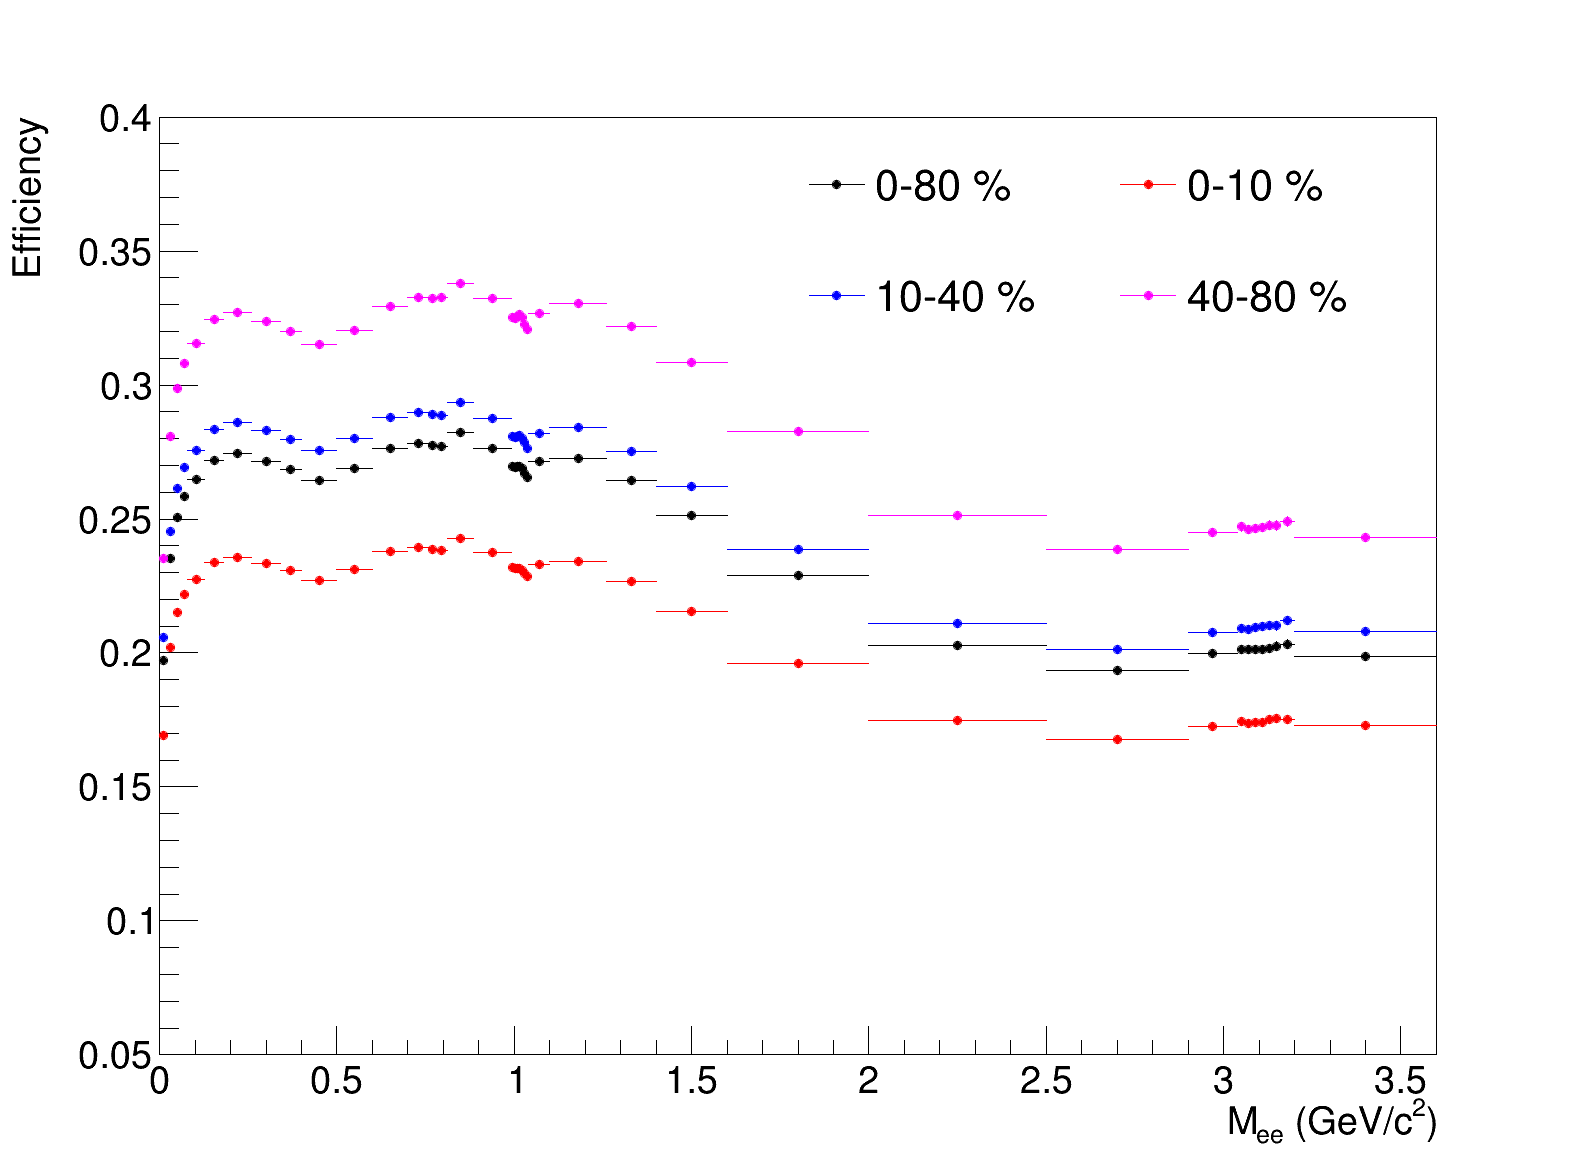
\includegraphics[width=0.75\textwidth,clip]{figures/Chapter4/Compare_PairEff.png}
    \end{center}
    \caption[不同中心度下的双电子重建效率]{\sNN = 54.4 GeV金-金对撞当中不同中心度下的双电子重建效率}
    \label{fig:Compare_PairEff}
\end{figure}

\subsection{接收度修正}
\label{chap:pair_acc}

在上一小节当中我们提到了STAR的接收度,如果我们要将STAR的测量结果和其他实验当中的结果进行比较,我们需要做的是要将STAR的结果修正到全空间当中去,消除STAR接收度的影响。而STAR的接收度修正因子可以通过和双电子效率类似的方式计算得到。计算方法如式\ref{eq:STAR_acc}所示。图\ref{fig:Accep_VP}\sNN = 54.4 GeV金-金对撞当中通过虚光子作为输入计算得到的STAR接受度修正因子。
\begin{equation}
    \label{eq:STAR_acc}
    f_{STAR acc.} = \frac{nPairs(p_T^{e} > 0.2~{\rm GeV/c} \&\& |Y_{ee} < 1| \&\& |\eta_e| < 1)}{nPairs}
\end{equation}
\begin{figure}[htb]
    \begin{center}
    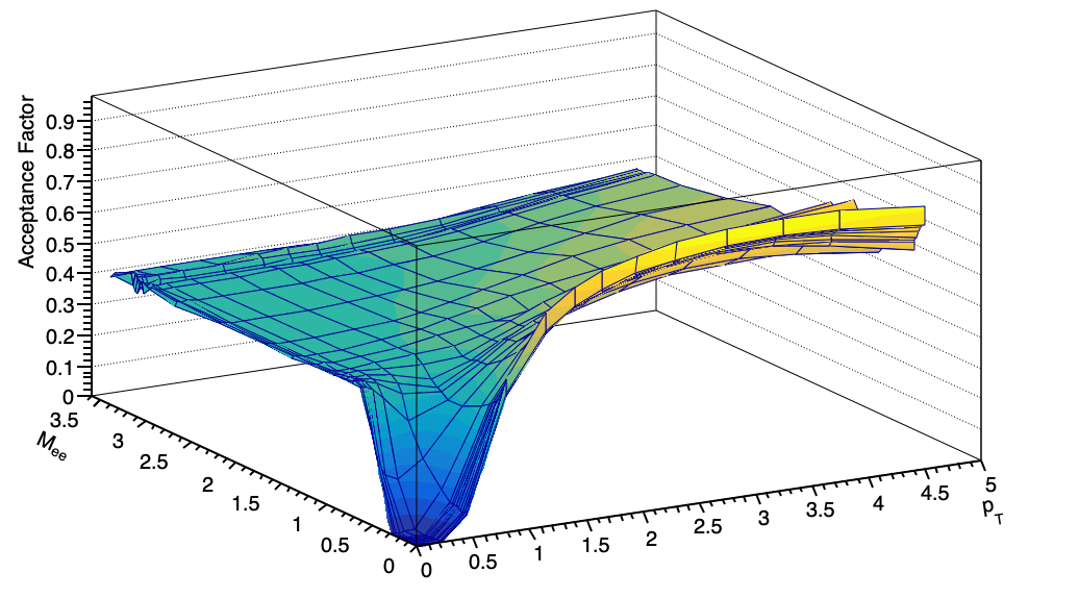
\includegraphics[width=0.75\textwidth,clip]{figures/Chapter4/Accep_VP.png}
    \end{center}
    \caption[通过虚光子作为输入计算得到的STAR接受度修正因子]{\sNN = 54.4 GeV金-金对撞当中通过虚光子作为输入计算得到的STAR接受度修正因子}
    \label{fig:Accep_VP}
\end{figure}
